\documentclass[sigconf]{acmart}

% ---- remove ACM boilerplate: copyright box, reference block, conference header ----
\settopmatter{printacmref=false, printccs=false, printfolios=true}
\setcopyright{none}
\renewcommand\footnotetextcopyrightpermission[1]{}
\acmDOI{}
\acmISBN{}
\acmConference{}{}{}

\usepackage{amsmath}
\usepackage{booktabs}
\newcommand{\core}{\textsc{CoRE}}
\setlength{\emergencystretch}{1.5em}

\begin{document}

\title{Which Condition Fits? An Empirical Evaluation of Multi-Label Diagnosis from Symptom Descriptions}
\titlenote{Code, data, and all results: \href{https://github.com/eduardokdp/Which-Condition-Fits-}{github.com/eduardokdp/Which-Condition-Fits-}. Reproduce every number, table and figure with \texttt{bash reproduce\_m4.sh} from the repository root.}

\author{Niyaaz Baines, Eduardo Kallina de Paula, Thiago Vasconcelos Pinheiro Lopes, and Priyanshkumar Ghanshyambhai Patel}
\affiliation{\institution{University of Victoria, Canada}}
\email{{nbaines, ekallinadepaula, thiagovplopes, priyanshkumarghansh1}@uvic.ca}

\renewcommand{\shortauthors}{Baines, Kallina de Paula, Lopes, and Patel}

\begin{abstract}
We evaluate \core{}, an order-averaged classifier chain that assigns a primary condition and any co-occurring ones (ADHD, anxiety, depression) to a self-reported symptom description. On 1,050 public Reddit posts with weak multi-label targets, every method is tuned by 5-fold cross-validation on shared folds and tested once on a held-out 20\%. \core{} has the highest macro-F1 (0.755) and AUC (0.865), but the 95\% bootstrap intervals of its leads over a multiclass classifier and the other linear baselines include zero; it is significantly better than Naive Bayes and $k$-NN. Its advantage is concentrated on posts with several conditions (macro-F1 0.835 vs 0.612), at the cost of over-predicting anxiety with depression. Code and results: \href{https://github.com/eduardokdp/Which-Condition-Fits-}{github.com/eduardokdp/\allowbreak Which-Condition-Fits-}.
\end{abstract}


\maketitle
\pagestyle{plain}

\begin{table*}[t]
\caption{Test results. $\Delta$: \core{} minus method (macro-F1), $^\ast$ if the paired 95\% interval excludes 0; ML-rec.: recall on multi-condition posts; Lab.: labels per post (true 1.11).}\label{tab:results}
\vspace{-6pt}
\footnotesize
\begin{tabular}{@{}l@{\hspace{4pt}}cccccccccccc@{}}
\toprule
& \multicolumn{7}{c}{RQ1: all 210 test posts} & \multicolumn{5}{c}{RQ3: macro-F1 by subgroup (posts)} \\
\cmidrule(lr){2-8}\cmidrule(l){9-13}
Method & Macro-F1 [95\% CI] & $\Delta$ & AUC & Micro-F1 & Ham.$\downarrow$ & ML-rec. & Lab. & One {\scriptsize(187)} & Several {\scriptsize(23)} & Short {\scriptsize(86)} & Med. {\scriptsize(61)} & Long {\scriptsize(63)} \\
\midrule
\core{} & \textbf{.755} {\scriptsize[.715,.790]} & -- & \textbf{.865} & \textbf{.750} & .211 & .766 & 1.41 & .734 & \textbf{.835} & \textbf{.767} & \textbf{.759} & .701 \\
Multiclass LR & .727 {\scriptsize[.674,.778]} & +.029 & .863 & .725 & \textbf{.194} & .447 & 1.00 & \textbf{.743} & .612 & .740 & .744 & .625 \\
Binary relevance & .732 {\scriptsize[.677,.778]} & +.024 & .854 & .731 & .213 & .723 & 1.26 & .713 & .755 & .717 & .721 & \textbf{.705} \\
Chain (1 order) & .737 {\scriptsize[.696,.771]} & +.018 & .857 & .730 & .237 & \textbf{.787} & 1.51 & .711 & .811 & .743 & .750 & .663 \\
Linear SVM & .733 {\scriptsize[.684,.775]} & +.022 & .855 & .730 & .221 & .723 & 1.34 & .716 & .755 & .716 & .741 & .689 \\
Naive Bayes & .686 {\scriptsize[.638,.728]} & +.069$^\ast$ & .831 & .682 & .270 & .638 & 1.43 & .676 & .606 & .652 & .724 & .627 \\
$k$-NN & .630 {\scriptsize[.577,.680]} & +.125$^\ast$ & .778 & .632 & .303 & .702 & 1.36 & .605 & .703 & .581 & .668 & .531 \\
\bottomrule
\end{tabular}

\vspace{-6pt}
\end{table*}

\begin{figure*}[t]
\centering
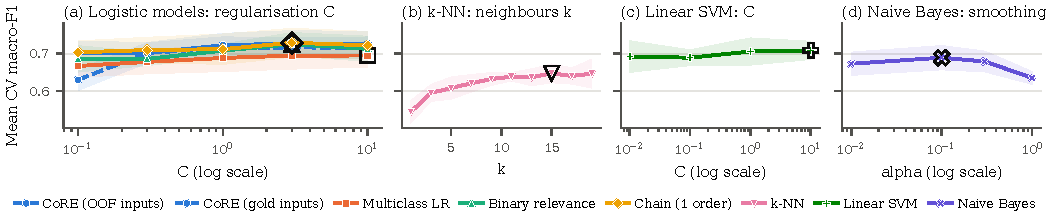
\includegraphics[width=\textwidth]{figures/rq2_sensitivity.pdf}
\vspace{-14pt}
\caption{RQ2: mean 5-fold CV macro-F1 ($\pm$1 s.d.); circled: selected setting.}\label{fig:rq2}
\vspace{-8pt}
\end{figure*}

\section{Introduction}
\core{} (Milestone~3) scores each condition with logistic-regression links averaged over all $3!$ chain orders on TF-IDF features of the masked text, reports the top condition as primary, and adds any other condition above a tuned threshold. We test its premise, that a description can fit several conditions, against standard classifiers.

\section{Research Questions}
\textbf{RQ1 (performance).} Does modelling co-occurring conditions beat single-condition and independent-label classifiers? If a one-label classifier does as well, \core{}'s extra modelling is not justified.
\textbf{RQ2 (sensitivity).} How do regularisation, $n$-grams and the chain's training inputs (out-of-fold or gold labels) affect \core{}, and how stable are the baselines?
\textbf{RQ3 (consistency).} Does the comparison hold for posts with one vs several conditions, and for short, medium and long posts, a measurable proxy for writing style?

\section{Benchmark Dataset}
We use 1,786 public Reddit posts (r/ADHD, r/Anxiety, r/depression) shared by two GitHub projects (Table~\ref{tab:data}); these communities match our conditions, and clinical corpora require data agreements we do not hold. After filtering we keep 350 posts per community. Targets combine the community with first-person diagnosis statements, as in SMHD \cite{cohan2018smhd}: 11.1\% of posts are multi-label, mostly anxiety with depression. Condition names are masked.

\begin{table}[t]
\caption{Benchmark dataset (bundled public sample).}\label{tab:data}
\vspace{-6pt}
\footnotesize
\begin{tabular}{@{}ll@{}}
\toprule
Posts (dev / test) & 1,050 (840 / 210); 350 per community \\
Labels ADHD / anx. / dep. & 358 / 428 / 383 positive \\
Label cardinality; multi-label & 1.11; 11.1\% \\
Co-occurring sets & anx+dep 97, ADHD+anx 11, ADHD+dep 7, all 2 \\
Features (dev TF-IDF) & 22,070 word $n$-grams; median 169 tokens \\
Removed in cleaning & 95 length, 2 duplicate, 639 over cap \\
Source; licence & GitHub; ADHD 2024 (MIT), anx./dep. 2025 (none) \\
\bottomrule
\end{tabular}

\vspace{-8pt}
\end{table}

\section{Baselines}
All methods get the same masked TF-IDF features (fitted on training data only), the same folds and, if multi-label, \core{}'s decision rule, so differences come from the scorer. \textbf{Multiclass LR}: softmax regression on the community label, one condition per post (the conventional framing). \textbf{Binary relevance} \cite{zhang2014review}: one logistic regression per condition, isolating label dependence. \textbf{Chain (1 order)} \cite{read2011classifier}: \core{} with the fixed order ADHD$\rightarrow$anxiety$\rightarrow$depression, isolating order averaging. \textbf{Linear SVM} \cite{joachims1998text}, one-vs-rest, scores mapped through a logistic function. \textbf{Complement Naive Bayes} \cite{rennie2003tackling}, one-vs-rest. \textbf{$k$-NN} \cite{cover1967nearest}: cosine distance, score = share of neighbours with the condition. All use scikit-learn 1.9.1 \cite{pedregosa2011scikit}. Transformers are excluded: they need a GPU and could not be tuned on equal terms.

\section{Evaluation Strategy and Metrics}
The data are split once (seed 42) into 80\% development and 20\% test, stratified on the label set \cite{sechidis2011stratification}. The development set gets 5 stratified folds, saved and reused by every method and configuration. Each round fits features and model on four folds minus a stratified 15\% that only tunes per-condition thresholds, and scores the fifth. Grids (Figure~\ref{fig:rq2}): $C$ and uni- vs bigrams for the logistic models, plus out-of-fold vs gold chain inputs for \core{}; $k$; SVM $C$; NB $\alpha$ (68 configurations, 340 fits). The best setting by mean CV macro-F1 is refitted on all development data and tested once.
\emph{Metrics.} Macro-F1 is primary: classes are balanced and each condition should count equally. Macro ROC-AUC measures ranking without thresholds; Hamming loss, recall on multi-condition posts and label-set confusion matrices show how errors arise. Accuracy is not used. Intervals and paired differences use 1,000 seeded bootstrap resamples \cite{efron1993bootstrap}.

\section{Results}


\textbf{RQ1.} \core{} ranks first on macro-F1 and AUC (Table~\ref{tab:results}), but its gains over the multiclass model (+0.029, interval $-0.012$ to $0.068$), binary relevance, the single-order chain and the SVM are not significant; only Naive Bayes and $k$-NN are significantly worse. The linear models' AUCs lie within 0.011: sharing features, they rank posts almost alike, so \core{}'s gain comes from its decisions (Figure~\ref{fig:conf}). The multiclass model never predicts a set, recovering 44.7\% of co-occurring conditions (\core{}: 76.6\%). In turn, \core{} labels 23 anxiety-only and 35 depression-only posts as both (1.41 labels per post), lowering its anxiety precision to 0.603 (multiclass 0.742) and raising Hamming loss. The chain's links explain this: they learn strongly negative weights between ADHD and the others ($-4.0$ to $-6.9$) but positive ones between anxiety and depression ($+1.82$, $+0.98$), the pair that co-occurs in 97 posts. $k$-NN is weakest: sparse TF-IDF neighbours share topic words across communities.

\begin{figure}[t]
\centering
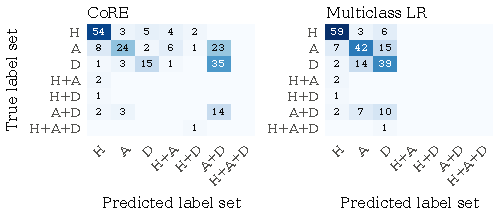
\includegraphics[width=\columnwidth]{figures/label_set_confusion.pdf}
\vspace{-16pt}
\caption{Test label sets. H: ADHD, A: anxiety, D: depression.}\label{fig:conf}
\vspace{-10pt}
\end{figure}

\textbf{RQ2.} \core{} is stable: for $C\ge0.3$ its CV macro-F1 stays within 0.688--0.727 (Figure~\ref{fig:rq2}), and the fold s.d.\ (about 0.03) exceeds the spread of the best linear models (0.695--0.729). It selects $C{=}3$, unigrams, out-of-fold inputs. Gold inputs never beat out-of-fold inputs at their best and collapse under strong regularisation (0.542 at $C{=}0.1$, bigrams): text weights shrink, so links lean on predecessor labels that are exact in training but noisy at test time. The single-order chain matches \core{} on the folds (0.729 vs 0.727): order averaging removes the arbitrary order rather than adding accuracy. $k$-NN gains up to $k{=}15$; Naive Bayes peaks at $\alpha{=}0.1$.



\textbf{RQ3.} The advantage is not uniform (Table~\ref{tab:results}, right). On the 23 posts with several conditions \core{} leads clearly (0.835 vs 0.612 for the multiclass model); on single-condition posts the multiclass model is slightly better (0.743 vs 0.734), as \core{} adds unneeded labels. Against the multiclass model, \core{} gains most on long posts (0.701 vs 0.625), where co-occurring labels are three times as frequent as in short ones (18.4\% vs 6.0\%).

\textbf{Threats to validity.} Weak labels measure agreement with communities and self-reports, not clinical diagnoses. The r/ADHD posts were collected in 2024 and the others in 2025, so source differences may help separate ADHD. With 210 test posts (23 with several conditions) intervals are wide. A larger single-collection corpus \cite{low2020natural} is supported by the code (\texttt{config/m4\_rmhd.yaml}) but was not run for this report.

\vspace{1mm}\noindent\textbf{Contributions.} Niyaaz: research questions, introduction; Thiago: dataset; Eduardo: baselines; Priyansh: evaluation strategy and metrics, experiments, results. \textbf{Use of AI} (Level D): Claude (Anthropic) drafted parts of the evaluation code and text; the authors reviewed, ran and revised them, and checked every reported number against the result files in the repository.

\bibliographystyle{ACM-Reference-Format}
\renewcommand{\bibfont}{\scriptsize}
\begin{thebibliography}{11}
\setlength{\itemsep}{0pt}
\bibitem{cohan2018smhd} A. Cohan et al. 2018. SMHD: A Large-Scale Resource for Exploring Online Language Usage for Multiple Mental Health Conditions. In \textit{Proc. COLING}. 1485--1497.
\bibitem{cover1967nearest} T. Cover and P. Hart. 1967. Nearest Neighbor Pattern Classification. \textit{IEEE Trans. Inf. Theory} 13, 1, 21--27.
\bibitem{efron1993bootstrap} B. Efron and R.~J. Tibshirani. 1993. \textit{An Introduction to the Bootstrap}. Chapman \& Hall.
\bibitem{joachims1998text} T. Joachims. 1998. Text Categorization with Support Vector Machines: Learning with Many Relevant Features. In \textit{Proc. ECML}. 137--142.
\bibitem{low2020natural} D.~M. Low et al. 2020. Natural Language Processing Reveals Vulnerable Mental Health Support Groups and Heightened Health Anxiety on Reddit During COVID-19. \textit{J. Med. Internet Res.} 22, 10, e22635.
\bibitem{pedregosa2011scikit} F. Pedregosa et al. 2011. Scikit-learn: Machine Learning in Python. \textit{JMLR} 12, 2825--2830.
\bibitem{read2011classifier} J. Read et al. 2011. Classifier Chains for Multi-label Classification. \textit{Machine Learning} 85, 3, 333--359.
\bibitem{rennie2003tackling} J.~D.~M. Rennie et al. 2003. Tackling the Poor Assumptions of Naive Bayes Text Classifiers. In \textit{Proc. ICML}. 616--623.
\bibitem{sechidis2011stratification} K. Sechidis, G. Tsoumakas, and I. Vlahavas. 2011. On the Stratification of Multi-label Data. In \textit{Proc. ECML PKDD}. 145--158.
\bibitem{zhang2014review} M.-L. Zhang and Z.-H. Zhou. 2014. A Review on Multi-Label Learning Algorithms. \textit{IEEE TKDE} 26, 8, 1819--1837.
\end{thebibliography}

\end{document}
